\documentclass[tikz, border=10pt]{standalone}
\usepackage{amsmath}

\begin{document}
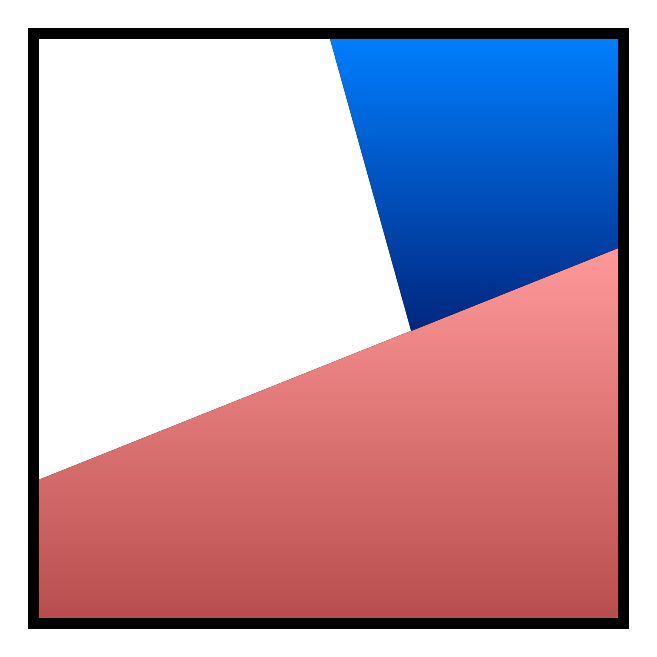
\begin{tikzpicture}[x=1.5cm, y=1.5cm]

    % ==========================================
    % 1. COORDINATES FOR GEOMETRY
    % ==========================================
    % Bottom Red/Pink region boundary intersects edges at (0, 1.2) and (5, 3.2)
    \coordinate (RedL) at (0, 1.2);
    \coordinate (RedR) at (5, 3.2);

    % Solid Blue region boundary 
    % Top intersects at x=2.5. Bottom intersects the red line at x=3.2
    \coordinate (SolidTop) at (2.5, 5);
    \coordinate (SolidBot) at (3.2, 2.48);

    % ==========================================
    % 2. CLIPPED REGIONS (Inside Pixel)
    % ==========================================
    \begin{scope}
        \clip (0,0) rectangle (5,5);

        % Bottom Region (Red/Salmon)
        \fill[top color=red!40!white, bottom color=red!60!black!70]
            (0,0) -- (5,0) -- (RedR) -- (RedL) -- cycle;

        % Top Right Region (Steel Blue)
        \fill[top color=blue!50!cyan, bottom color=blue!70!cyan!50!black]
            (SolidTop) -- (5,5) -- (5,3.2) -- (SolidBot) -- cycle;
    \end{scope}

    % ==========================================
    % 3. PIXEL BOUNDARY & TEXT
    % ==========================================
    % Thick black border for the pixel
    \draw[line width=4pt, black] (0,0) rectangle (5,5);

    % Corner Label "D"
    % \node[font=\Huge\rmfamily, text=black, anchor=north west, inner sep=8pt] 
    %     at (0, 5) {D};

\end{tikzpicture}
\end{document}